\section{Mathematical model}
\label{sec:model}
A numerical CFD model of the cross flow around a circular cylinder was prepared utilizing the OpenFOAM open-source CFD library \citep{OpenFOAM2007}, which is based on the finite volume method (FVM). In the following, we first list the flow governing equations and discuss the selected approach to the turbulence modeling. Next, we concentrate on the used computational mesh and problem boundary conditions. The section is concluded by listing the applied numerical methods and by a discussion of the solution independence with respect to the selected mesh resolution.

\subsection{Flow governing equations, turbulence modeling and boundary conditions}
\label{sub:flowEqs}
Let us denote the spatial domain corresponding to the geometry shown in Figure~\ref{fig:geom} as $\Omega$ and its boundary as $\partial\Omega$. Next, let $Q = (0,T]\times \Omega$ be the complete spatio-temporal computational domain. The flow in $Q$ is assumed to be governed by the standard set of the Navier-Stokes equations for an incompressible and isothermal flow of a Newtonian fluid, i.e.
\begin{equation}
\label{eq:nsEqs}
    \begin{array}{*1{>{\displaystyle}c}}
        \frac{\partial \bm{u}}{\partial t} + \nabla \cdot \left( \bm{u} \otimes \bm{u}\right) - \nabla \cdot \bm{T} = -\nabla \tilde{p} \\[0.2cm]
        \nabla \cdot \bm{u} = 0
    \end{array}\quad \forall (t,\bm{x})\in Q
\end{equation}
where $\bm{u}$ is the fluid velocity, $\tilde{p} = p/\rho$ is the kinematic pressure obtained by dividing the pressure $p$ by the fluid density $\rho$, which is assumed to be constant in $Q$. Finally, $\bm{T}$ is the viscous stress tensor.

Due to the computational costs, not all the flow scales in $Q$ are directly simulated. Instead, the turbulent flow is solved within the large eddy simulation (LES) framework in which $\bm{u}$ and $\tilde{p}$ are replaced by their filtered counterparts $\filtU$ and $\filtP$ and the stress tensor $\bm{T}$ is decomposed as 
\begin{equation}
\label{eq:stress}
    \bm{T} = \filtT + \sgsT\,,
\end{equation}
where $\filtT$ is the filtered, or resolved scale, strain rate tensor and $\sgsT$ is the unknown subgrid scale (SGS) stress tensor that represents the effects of SGS motion on the resolved LES fields \citep{yang2015}.

Furthermore, in order to correctly and efficiently account for the spatial computational domain $\Omega$ being relatively large compared to the region of interest containing the two planes of measurement, we use a hybrid LES-RANS turbulence model introduced by \citet{strelets2001}. Within this approach, known as the detached eddy simulation (DES), a single turbulence model is used that acts as a subgrid scale model where the grid resolution is high enough and as a RANS model in the regions where it is not \citep{strelets2001}.

In the particular DES formulation used in the present work the applied turbulence model is the $k-\omega$ shear stress transport (SST) model by \citet{menter1992} as reformulated by \citet{hellsten1997} and summarized in \citep{menter2003}. The closure of the problem~\eqref{eq:stress} is based on a solution of two additional transport equations for the unknown modeled turbulence kinetic energy ($k$) and the specific dissipation rate ($\omega$). The model equations for incompressible flow are
\begin{equation}
\label{eq:kOmegaSSTDES}
    \begin{array}{*1{>{\displaystyle}c}}
        \frac{\partial {k}}{\partial t} + \nabla \cdot \left( \bm{u}\, k\right) = \tilde{P}_{k} - \beta^{*}k\,\omega\,F_{\mathrm{DES}} + \nabla \cdot \left(\left(\nu + \sigma_{k}\nu_{t}\right)\nabla k\right)\\[0.2cm]
        \frac{\partial {\omega}}{\partial t} + \nabla \cdot \left( \bm{u}\, \omega\right) = \alpha\,S^{2} - \beta\,\omega^{2} + \nabla \cdot \left(\left(\nu + \sigma_{\omega}\nu_{t}\right)\nabla \omega\right) + 2\left(1-F_{1}\right)\sigma_{w2}\frac{1}{\omega}\nabla k \cdot \nabla \omega\\[0.2cm]
        \quad \forall (t,\bm{x})\in Q
    \end{array}
\end{equation}
where the constants and parameters $\tilde{P}_{k},\,\beta^{*},\,\sigma_{k},\,\alpha,\,S,\,\beta,\,F_{1}$ and $\sigma_{w2}$ may be found for example in \citep{hellsten1997} or \citep{menter2003}. The function $F_{\mathrm{DES}}$ accounts for the DES modification to the standard $k-\omega$ SST model and is defined as
\begin{equation}
\label{eq:FDES}
    F_{\mathrm{DES}} = \max\left\{\frac{\ell_{t}}{C_{\mathrm{DES}}\Delta},1 \right\},\,\ell_{t} = \frac{\sqrt{k}}{\beta^{*}\omega},\,\Delta = \max\{\Delta_{x},\Delta_{y},\Delta_{z}\},\,C_{\mathrm{DES}} = 0.61
\end{equation}
with $\ell_{t}$ being the local turbulent length, $\Delta$ the local maximum grid spacing for a cartesian mesh and $C_{\mathrm{DES}}$ the model calibration constant. Note that the model as listed in~\eqref{eq:kOmegaSSTDES} and~\eqref{eq:FDES} may be used even on unstructured non-cartesian meshes. The only modification required lies in correctly estimating $\Delta$ on such meshes.

% Note (MI): we might have to check this and make it consistent with the OpenFOAM formulation
% https://www.openfoam.com/documentation/guides/latest/doc/guide-turbulence-des-k-omega-sst-des.html
% or it even might be already consistent... I just didn't check it

\begin{table}[htbp]
\hspace*{-2.0cm}
{
\begin{tabular}{lclclc}
\toprule
    Boundary & Conditions & Boundary & Conditions & Boundary & Conditions \\
\midrule
    \multirow{4}{*}{inlet}
    &
    $\bm{u} = (u_{\mathrm{in}},0,0)^{\mathrm{T}}$ & \multirow{4}{*}{outlet} &  $\bm{n} \cdot \bm{u} = (0,0,0)^{\mathrm{T}}$ & \multirow{4}{*}{cylinder} & $\bm{u} = (0,0,0)^{\transp}\leftarrow$ \textit{no-slip}\\
    &
    $\bm{n}\cdot\nabla p = 0$ & & $p = 0$ & & $\bm{n}\cdot\nabla p = 0$\\
    &
    $k = k_{0} \leftarrow I = 0.2\,\%$ & & $\bm{n}\cdot\nabla k = 0$ & & $k = 0$\\
    &
    $\omega = \omega_{0} \leftarrow I = 0.2\,\% $ & & $\bm{n}\cdot \nabla\omega = 0$ & & $\bm{n}\cdot \nabla\omega = 0$\\
\midrule
    \multirow{4}{*}{virtual walls}
    &
    $\bm{u}\leftarrow$ \textit{slip} & \multirow{4}{*}{walls} & $\bm{u} = (0,0,0)^{\transp}\leftarrow$ \textit{no-slip}\\
    &
    $\bm{n}\cdot\nabla p = 0$ & & $\bm{n}\cdot\nabla p = 0$\\
    &
    $\bm{n}\cdot\nabla k = 0$ & & $k \leftarrow$ wall function\\
    &
    $\bm{n}\cdot\nabla \omega = 0$ & & $\omega \leftarrow$ wall function\\
\bottomrule
\end{tabular}
}
\caption{Applied boundary conditions. The \textit{virtual walls} are shown in red in Figure~\ref{fig:geom}.}
\label{tab:BC}
\end{table}

The used boundary conditions are mostly standard and are summarized in Table~\ref{tab:BC}. However, it was necessary to resolve the geometric discrepancy between the experiment and simulation, shown in Figure~\ref{fig:geom}. The flow field at the inlet is well defined with $u_{\mathrm{in}} = 5\,\mathrm{m\,s^{-1}}$ and $I =  0.2\,\%$. Still, in the simulation, the inlet needed to be moved upstream, see the red (\textit{virtual}) walls in Figure~\ref{fig:geom}a. To keep the flow uniformity at the contact with the cylinder, the \textit{slip} boundary condition,
\begin{equation}
\label{eq:slipBC}
    \bm{u}\cdot \bm{n} = 0\quad \text{ and }\quad \bm{t}_{\mathrm{w},t} = \bm{t}_{\mathrm{w}} - \left(\bm{n}\cdot \bm{t}_{\mathrm{w}} \right)\bm{n} = 0\,,
\end{equation}
where $\bm{t}_{\mathrm{w}}$ is the wall stress vector, is applied at the \textit{virtual walls}. Finally, note that although the wall functions are used for the turbulence variables at the test section walls, the mesh resolution is such that they are effectively turned-off for most of the test-section and affect the flow solution only downstream from the region of interest.

\subsection{Computational mesh}
\label{sub:meshAndBC}
Let $\Omega^{h}$ mark the finite volume spatial discretization of $\Omega$, i.e. the computational mesh. The mesh was constructed such that the region of interest
\begin{equation}
    \label{eq:RoI}
    {\mathrm{RoI} = \{(x_r,y_r,z_r)\in\mathbb{R}^{3}:x_r\in [0,7],\,y_r\in[-2,2],z_r=\in[-3,3]\}}
\end{equation}
as well as the parts of $\Omega$ directly affecting the flow in RoI comprise a structured hex-dominant grid with the resolution sufficient to fully simulate all the relevant flow scales. On the other hand, the main purpose of the computational domain outside of RoI is to provide physically correct boundary conditions at the RoI boundaries. Thus, the mesh in these regions is coarsened and the flow there is simulated using the $k-\omega_{\mathrm{SST}}$ unsteady RANS model.

\begin{figure}[htbp]
    \hspace*{-1.5cm}
    % \begin{tikzpicture}
    %     \node (mesh) at (0,0) {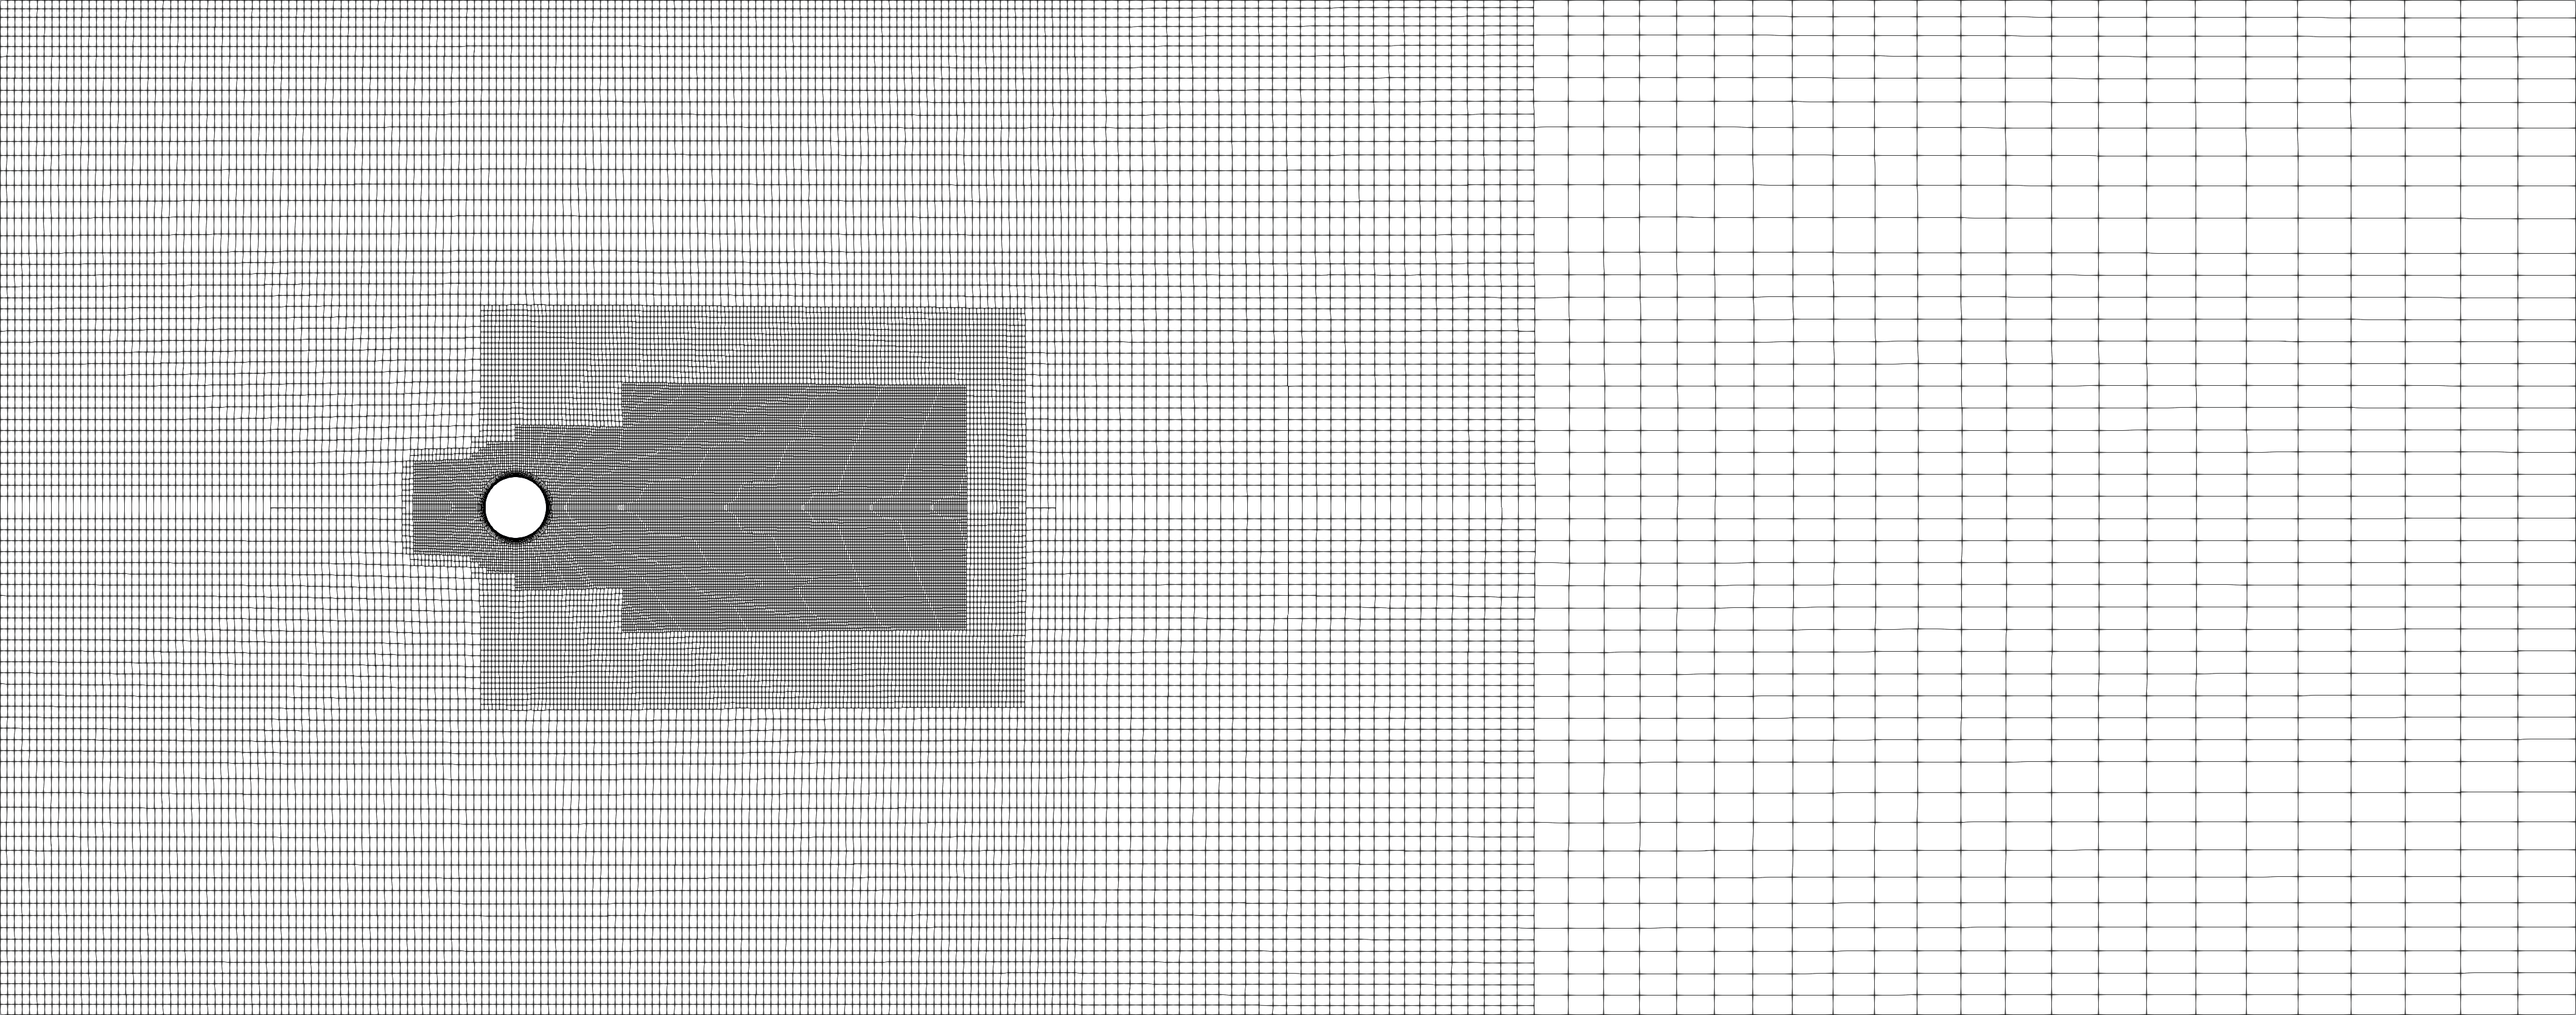
\includegraphics[width=0.9\auxWidth]{\myImages/meshSideViewV3Trp.png}};
        
    %     \draw[thick,red] (-4.63,-1.0) rectangle (-2.0,1.0);
        
    %     DNS regions
    %     \draw[thick,blue] (-5.0,-0.2) -- (-1.8,-0.9) -- (-1.8,0.9) -- (-5.0,0.2) -- cycle;
    %     \draw[thick,blue]   (-0.45\auxWidth,2.9) -- (-1.5,2.7) -- (-1.5,2.9) -- cycle;
    %     \draw[thick,blue]   (-0.45\auxWidth,-2.9) -- (-1.5,-2.7) -- (-1.5,-2.9) -- cycle;
    %     \node[blue,fill=white,draw=blue] at (-2.7,-0.34) {DNS};
        
    %     LES regions
    %     %~ \draw[thick,green!70!black] (-1.5,2.7) -- (0.45\auxWidth,2.5) -- (0.45\auxWidth,1.5) -- cycle;
    %     \draw[thick,green!70!black] (-1.5,2.7) -- (1.4,2.5) -- (1.4,-2.5) -- (-1.5,-2.7);
    %     \draw[thick,green!70!black] (-0.45\auxWidth,-2.9) -- (-0.45\auxWidth,2.9);{}
    %     \node[green!70!black,fill=white,draw=green!70!black] at (0.9,-2.25) {LES};
        
    %     RANS/URANS regions
    %     \draw[thick,brown]  (-1.5,2.9) -- (0.45\auxWidth,2.9) -- (0.45\auxWidth,-2.9) -- (-1.5,-2.9);
    %     \node[brown,fill=white,draw=brown] at (0.365\auxWidth,-2.55) {RANS/URANS};
        
    %     plane of symmetry
    %     \draw[thick,dashdotted] (-0.45\auxWidth,0) -- (0.45\auxWidth,0) node[above=-0.07cm,midway] {plane of symmetry};
        
    %     layers
    %     \node[above left=0.5cm and 0.3cm,fill=white,draw=black,anchor=east] (layers) at (mesh.east) {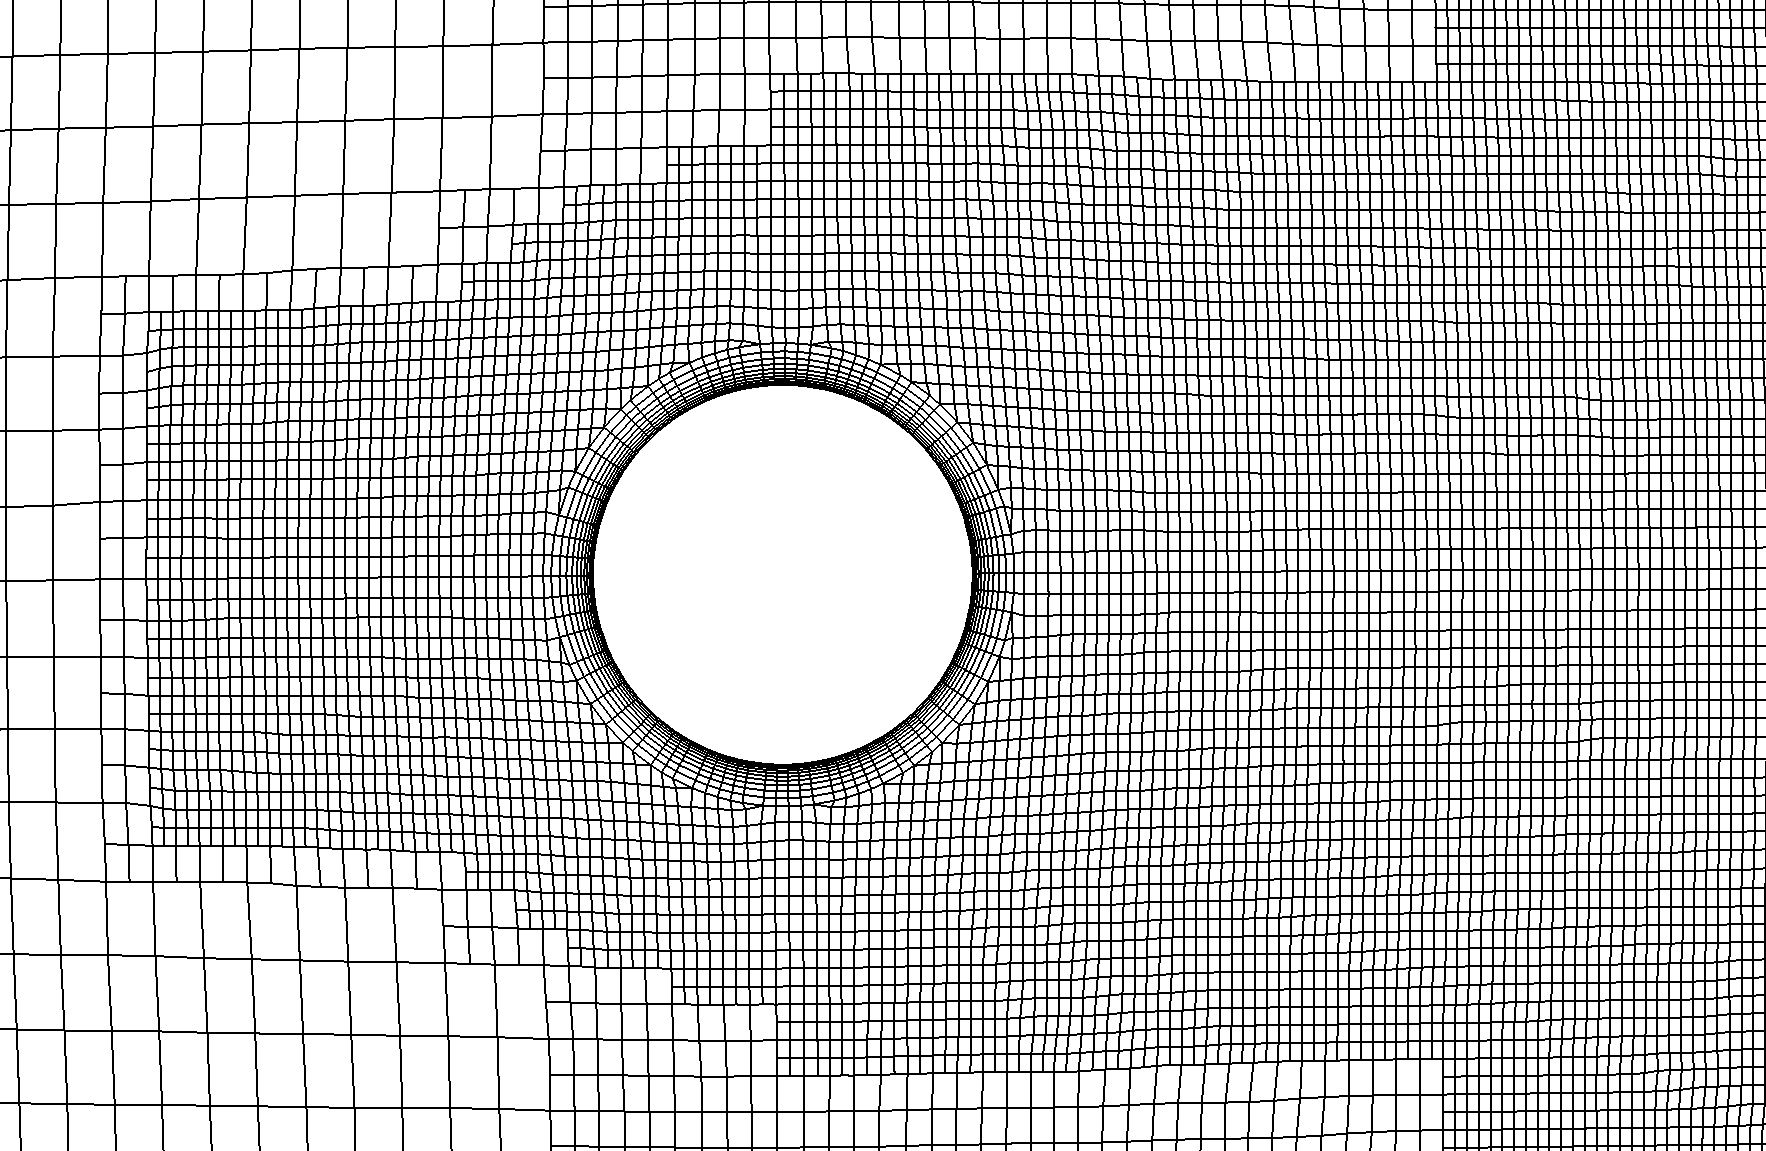
\includegraphics[width=0.31\auxWidth]{\myImages/meshSideViewDetCylV3Trp.png}};
    %     \node[anchor=south,above=0.05cm,fill=white] at (layers.south) {detail of $\Omega^{h}$ close to the cylinder};
        
    %     dimensions
    %     \draw[<->] (-0.45\auxWidth,3.3) -- (0.45\auxWidth,3.3) node[above,midway] {$L = 42.0 \,d$}; 
    %     \draw[<->] (-0.45\auxWidth,-3.3) -- (-4.63,-3.3) node[below,midway] {$L_{\mathrm{in}} = 8.5 \,d$}; 
    %     \draw[<->] (-4.63,-3.3) -- (0.45\auxWidth,-3.3) node[below,midway] {$L_{\mathrm{w}} = 33.5 \,d$}; 
    %     \draw[<->] (0.45\auxWidth,-2.9) -- (0.45\auxWidth,2.9) node[below,midway,rotate=90] {$W = 16.7 \,d = 25\,\mathrm{cm}$};
        
    % \end{tikzpicture}
    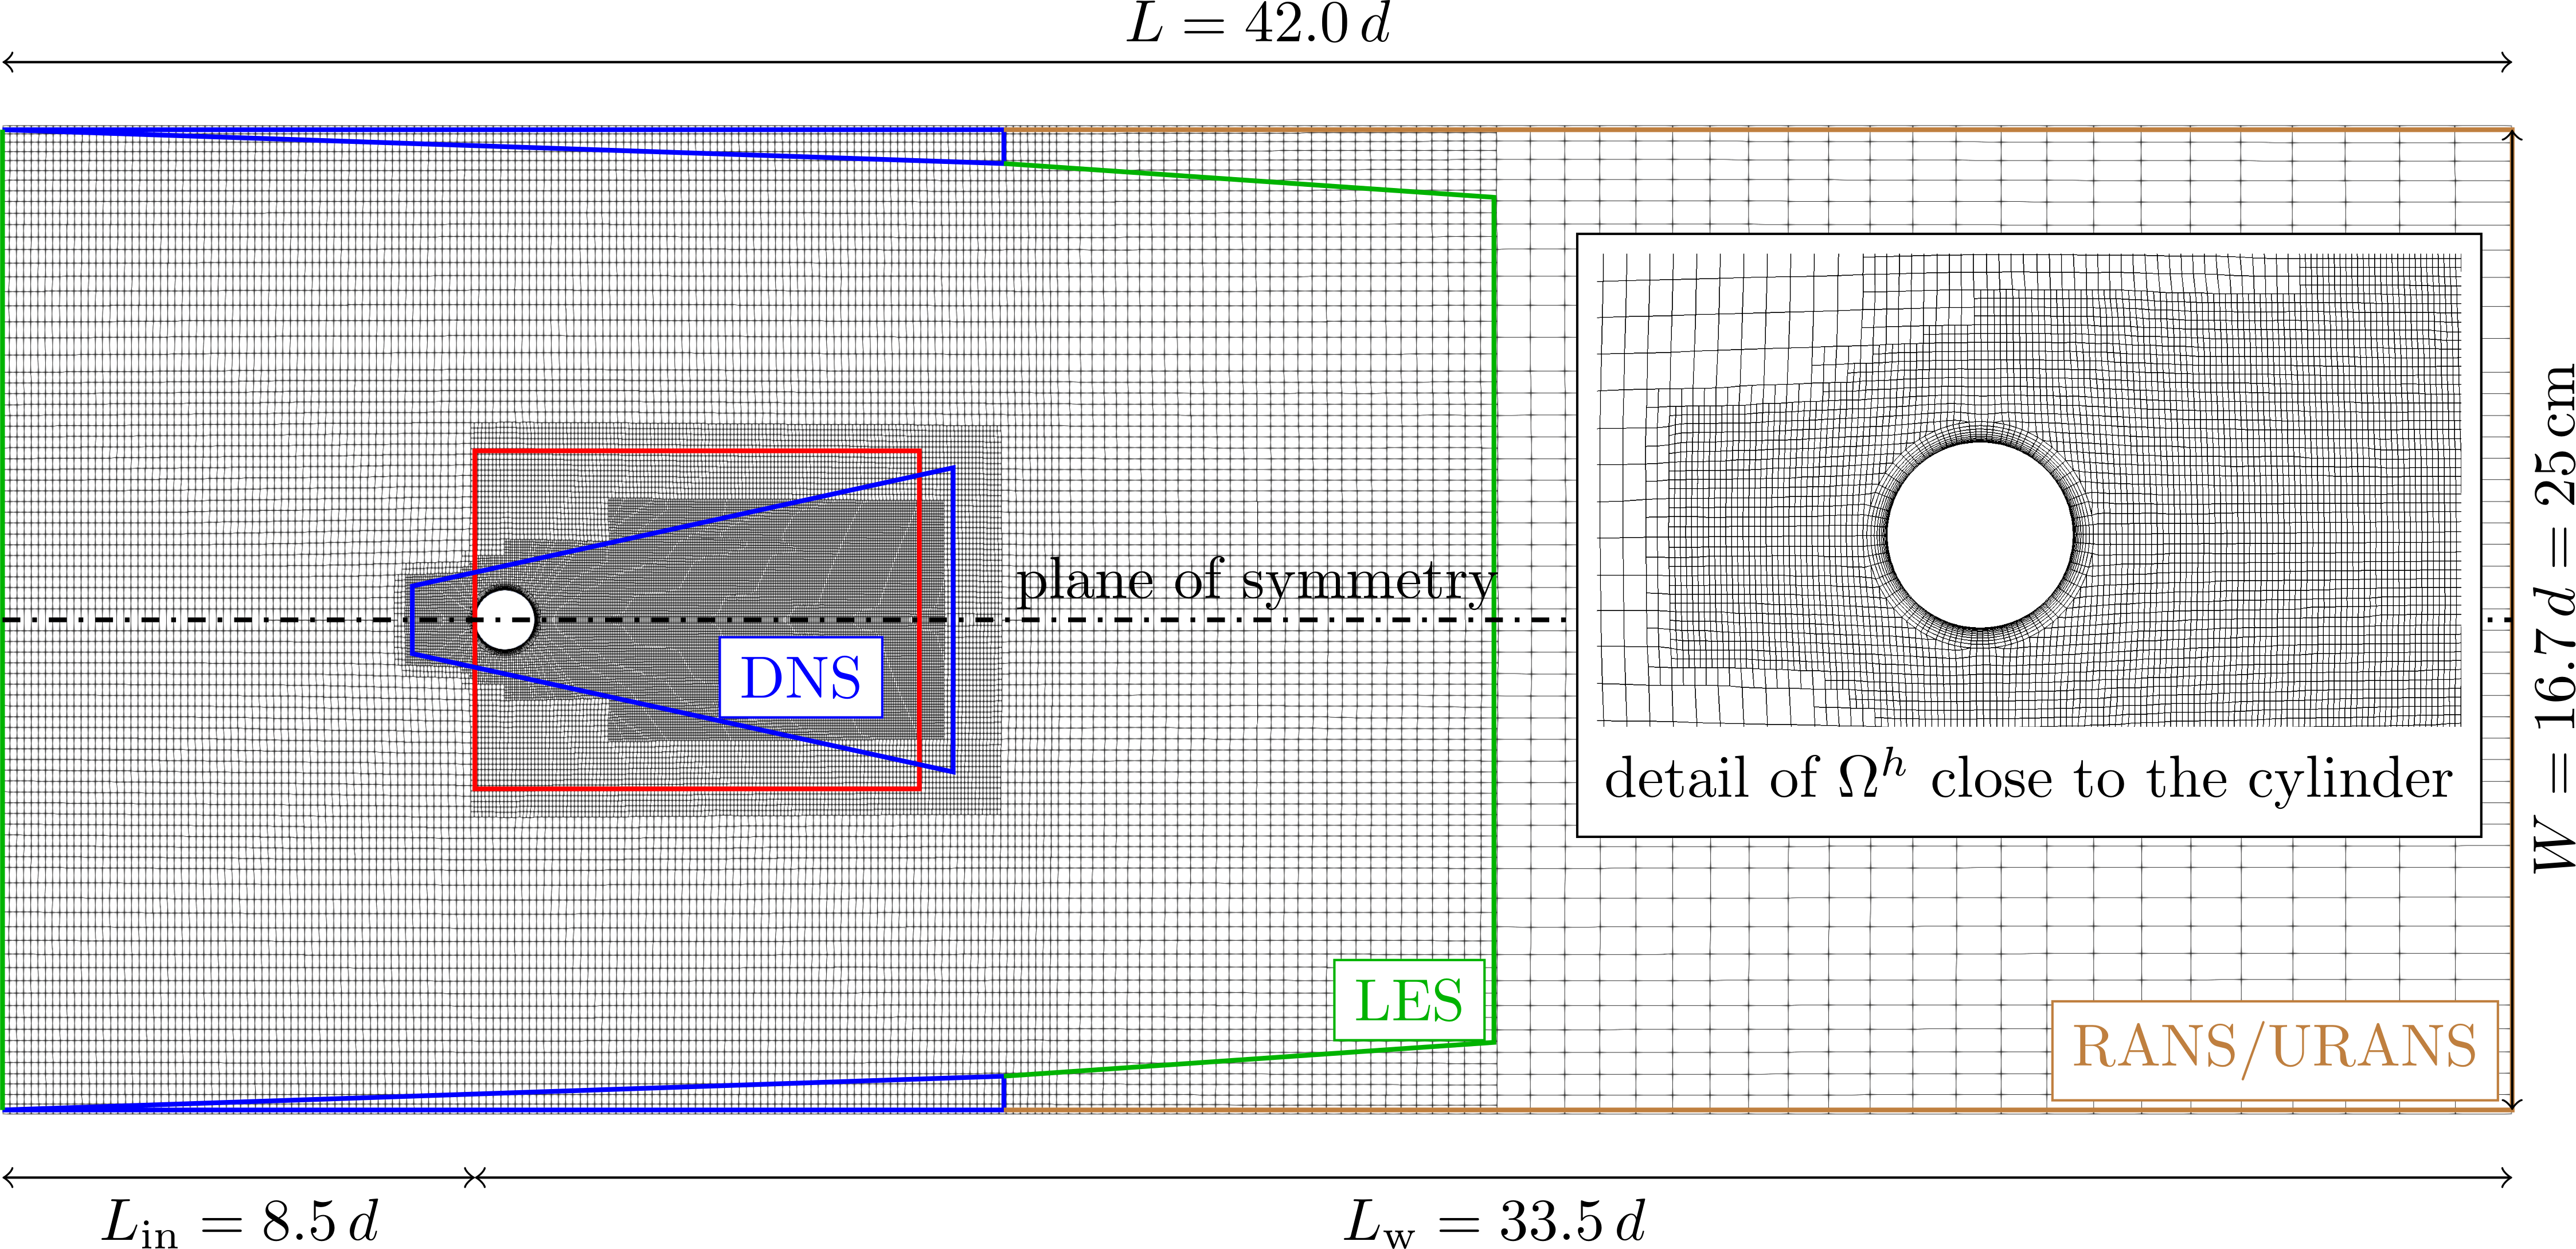
\includegraphics[width=0.98\textwidth]{02_images/00_export/figure2.png}
    \caption{Cut through the computational mesh ($\Omega^{h}$) in $x-y$ plane, which contains the streamwise plane of measurement (PoM1). Regions of activity for different turbulence models are highlighted. The region of interest (RoI) is outlined in red.}
    \label{fig:compMesh}
\end{figure}

The overall mesh structure in the $x-y$ plane is shown in Figure~\ref{fig:compMesh}. Note the high mesh resolution directly in front of the cylinder and the grid refinement towards the test section walls as indicated by the blue regions in Figure~\ref{fig:compMesh}. The high-resolution mesh in front of the bluff body is necessary to correctly resolve the pressure field, which affects the flow separation. As for the regions close to the test section walls, let us recall that at $x = 0$;
\begin{inparaenum}[(i)]
 \item in experiment, there is a transition between the inlet nozzle and the test section walls, and
 \item in simulation, there is a transition between the \textit{virtual wall} posing no tangential resistance to the flow and a standard wall.
\end{inparaenum}
Consequently, close to $x = 0$, there is a boundary layer separation on walls both in the experiment and simulation. At the studied $\Rey = 4185$, this so-called wall effect influences the wake behind the cylinder already towards the end of the region of interest and as such, it needs to be correctly resolved.

The mesh structure with respect to the $z$ axis direction is simpler than the one in the $x-y$ plane. Once more, the mesh is refined towards the test section walls. The most refined (DNS) region, which is shown in blue in Figure~\ref{fig:compMesh}, stretches between $z_{r} > -2$ and $z_{r} < 2$ and is encapsulated within the one level less refined region visible in Figure~\ref{fig:compMesh} in a way that this encapsulating region is roughly {$15\,\%$} wider than the region of interest. Finally, as shown in the detail of the mesh close to the cylinder in Figure~\ref{fig:compMesh}, ten surface layers, with the thickness increasing with the distance from the cylinder, were added onto the cylinder model in order to catch the flow separation as correctly as possible.


\subsection{Numerical methods and mesh size independence}
\label{sub:numerics}
The flow governing equations were solved within {via} the finite volume method (FVM) {variant implemented in the OpenFOAM C++ library \citep{OpenFOAM2007}}. In the ideal case, FVM is second order accurate in space. However, application of the second order accurate discretization to convection terms in~\eqref{eq:nsEqs} and in~\eqref{eq:kOmegaSSTDES} leads to numerical instability even at low $\Rey$~\citep{moukalled2016}. Thus, {high-resolution} schemes switching between second and first order accuracy have been applied to the terms $\nabla \cdot \left( \bm{u} \otimes \bm{u}\right)$, $\nabla \cdot \left( \bm{u}\, k\right)$ and $\nabla \cdot \left( \bm{u}\, \omega\right)$ in~\eqref{eq:nsEqs} and~\eqref{eq:kOmegaSSTDES}, respectively. In particular, a variant of a second order upwind scheme with an explicit correction based the local gradient was used for the velocity term. For the turbulence terms, the self-filtered central differencing scheme \citep{zhu1991} was applied. The remaining spatial discretization terms were treated with the second order accuracy. Finally, the temporal integration was performed utilizing an off-centered variant of the Crank-Nicolson method \citep{crankNicolson1947}, which is close to second order accurate with respect to time.

The simulation was carried out utilizing adaptive time-stepping with the time step limited by the maximal allowed Courant number of $0.5$. The overall solution method of equations~\eqref{eq:nsEqs} and~\eqref{eq:kOmegaSSTDES} was based on the PIMPLE algorithm as implemented in OpenFOAM \citep{OpenFOAM2007}. On each time level, the system was iteratively solved until the relative residual in pressure fell under $10^{-4}$.

\begin{figure}[htbp]
    \centering
    % \begin{tikzpicture}
	\begin{axis}[
			width=0.75\linewidth,
			height = 4cm,
			scale only axis,
			name=plot1,
			xlabel=$x_r$,
			ylabel={$u_r$ [-]},
			%~ ymode=log,
			%~ xmode=log,
			ymax = 0.8,
			xmin = 0.5,
			ymin = -0.5,
			xmax = 7,
			ytick pos=left,
			mark size=4pt,    
			line width = 0.9pt,
			%~ legend style={at={(axis cs:6,2)},anchor=south west},				
		]
		% \addplot [color = black!50,mark =none]table [y=u_x,x =x]{\myGraphs/msIndData/expLineResV1.dat};\label{uxExp}
		\addplot [color = blue,mark =none]table [col sep=comma, y expr=(\thisrow{U:0})/5,x expr = {(\thisrow{Points:0})/0.015}]{\myGraphs/msIndData/mS_40p_U.csv};\label{mesh40U}
		\addplot [color = red,mark =none]table [col sep=comma, y expr=(\thisrow{U:0})/5,x expr = {(\thisrow{Points:0})/0.015}]{\myGraphs/msIndData/mS_50p_U.csv};\label{mesh50U}
		\addplot [color = green,mark =none]table [col sep=comma, y expr=(\thisrow{U:0})/5,x expr = {(\thisrow{Points:0})/0.015}]{\myGraphs/msIndData/mS_75p_U.csv};\label{mesh70U}
		\addplot [color = black,mark =none]table [col sep=comma, y expr=(\thisrow{U:0})/5,x expr = {(\thisrow{Points:0})/0.015}]{\myGraphs/msIndData/bCyl_l_3_U.csv};\label{mesh100U}
		% \addplot [color = magenta,mark =none]table [col sep=comma, y expr=(\thisrow{U:0})/5,x expr = {(\thisrow{Points:0})/0.015}]{\myGraphs/msIndData/bCyl_l_3V2_U.csv};\label{mesh110U}
		% \addplot [color = orange,mark =none]table [col sep=comma, y expr=(\thisrow{U:0})/5,x expr = {(\thisrow{Points:0})/0.015}]{\myGraphs/msIndData/mS_120p_U.csv};\label{mesh120U}
		%~ \addplot [color = red,mark =none]table [y=U_x_ms_50_U,x =z_ms_50_U]{\myGraphs/onLineMSV2.dat};\label{mesh50U}
		%~ \addplot [color = green,mark =none]table [y=U_x_ms_70_U,x =z_ms_70_U]{\myGraphs/onLineMSV2.dat};\label{mesh70U}
		%~ \addplot [color = black,mark =none]table [y=U_x_ms_100_U,x =z_ms_100_U]{\myGraphs/onLineMSV2.dat};\label{mesh100U}
		%~ \addplot [color = black,mark =none]table [y=U_x_ms_100_U,x =z_ms_120_U]{\myGraphs/onLineMSV2.dat};\label{mesh100U}
		\coordinate (top) at (rel axis cs:0,1);
		\end{axis}
    \begin{axis}[
			width=0.75\linewidth,
			height = 4cm,
			scale only axis,
			xlabel=$x_r$,
			%~ ylabel={\textcolor{red}{TKE}},
			ylabel={$k$ [-]},
			%~height=\figHeight,
			scale only axis,
			%~ xmin=0,
			%~ xmax=600,
			xmin=0.5,
			xmax=7,
			ymin=0,
			ymax = 0.3,
			%~ ymax=1000,
			hide x axis,
			line width = 0.9pt,
			axis y line*=right,
			%~ axis line style={red},
			%~ axis y label/.append style ={red},
			%~ ytick label/.append style = {red},
			%~ ylabel={$y_{\mathrm{NO}},\,y_{\mathrm{N_{2}O}} \mathrm{\,[ppm]}$},
			mark size=2.5pt, 
        ]
		% \addplot [color = black!50,mark =none,dashed]table [y=k,x =x]{\myGraphs/msIndData/expLineResKV1.dat};\label{kExp}
        \addplot [color = blue,mark =none,dashed]table [col sep=comma, y expr=(\thisrow{k}),x expr = {(\thisrow{Points:0})/0.015}]{\myGraphs/msIndData/mS_40p_k.csv};\label{mesh40k}
        \addplot [color = red,mark =none,dashed]table [col sep=comma, y expr=(\thisrow{k}),x expr = {(\thisrow{Points:0})/0.015}]{\myGraphs/msIndData/mS_50p_k.csv};\label{mesh50k}
        \addplot [color = green,mark =none,dashed]table [col sep=comma, y expr=(\thisrow{k}),x expr = {(\thisrow{Points:0})/0.015}]{\myGraphs/msIndData/mS_75p_k.csv};\label{mesh70k}
        \addplot [color = black,mark =none,dashed]table [col sep=comma, y expr=(\thisrow{k}),x expr = {(\thisrow{Points:0})/0.015}]{\myGraphs/msIndData/bCyl_l_3_k.csv};\label{mesh100k}
		% \addplot [color = magenta,mark =none,dashed]table [col sep=comma, y expr=(\thisrow{k}),x expr = {(\thisrow{Points:0})/0.015}]{\myGraphs/msIndData/bCyl_l_3V2_k.csv};\label{mesh110k}
        % \addplot [color = orange,mark =none,dashed]table [col sep=comma, y expr=(\thisrow{k}),x expr = {(\thisrow{Points:0})/0.015}]{\myGraphs/msIndData/mS_120p_k.csv};\label{mesh120k}

		\coordinate (bot) at (rel axis cs:1,0);
\end{axis}

    \matrix[
        matrix of nodes,
        anchor=south,
        draw,
        inner sep=0.2em,
        %~ thick,
        fill=white,
      ]at([xshift=0,yshift=0.2cm]plot1.south)
      {
        %~ \ref{100}& CFD old &[5pt]\\
        %~ \ref{60}& XPF - reac, wall&[5pt]\\
		% \ref{uxExp}& exp U &
        % \ref{mesh100U}& $u$ &
        \ref{mesh40U}& 3.5M cells &
        % \ref{uxExp}& $U$ exp &[5pt]\\
        \ref{mesh50U}& 5.0M cells & \\
        \ref{mesh70U}& 7.4M cells &
        \ref{mesh100U}& 8.3M cells & 
		% \ref{mesh110U}& 110 U &
        % \ref{mesh120U}& 120 U\\
		% \ref{kExp}& exp k &
        % \ref{mesh100k}& $k$ &
        % \ref{mesh40k}& 40 k &
        % % \ref{uxExp}& $U$ exp &[5pt]\\
        % \ref{mesh50k}& 50 k &
        % \ref{mesh70k}& 75 k &
        % \ref{mesh100k}& 100 k &
		% \ref{mesh110k}& 110 k &
        % \ref{mesh120k}& 120 k
		\\
%        \ref{legendNoReact}& $\mathrm{thermic\ no\ reaction\ heat}$&[5pt]
        \\};
	\matrix[
        matrix of nodes,
        anchor=east,
        draw,
        inner sep=0.2em,
        %~ thick,
        fill=white,
      ]at([xshift=-0.2cm,yshift=0cm]plot1.east)
      {
        %~ \ref{100}& CFD old &[5pt]\\
        %~ \ref{60}& XPF - reac, wall&[5pt]\\
		% \ref{uxExp}& exp U
		
        \ref{mesh100U}& $u_r$ \\
		% \ref{mesh110U}& 110 U &
        % \ref{mesh120U}& 120 U\\
		% \ref{kExp}& exp k &
        \ref{mesh100k}& $k$ &
        % \ref{mesh40k}& 40 k &
        % % \ref{uxExp}& $U$ exp &[5pt]\\
        % \ref{mesh50k}& 50 k &
        % \ref{mesh70k}& 75 k &
        % \ref{mesh100k}& 100 k &
		% \ref{mesh110k}& 110 k &
        % \ref{mesh120k}& 120 k
		\\
%        \ref{legendNoReact}& $\mathrm{thermic\ no\ reaction\ heat}$&[5pt]
        \\};
	\end{tikzpicture}

    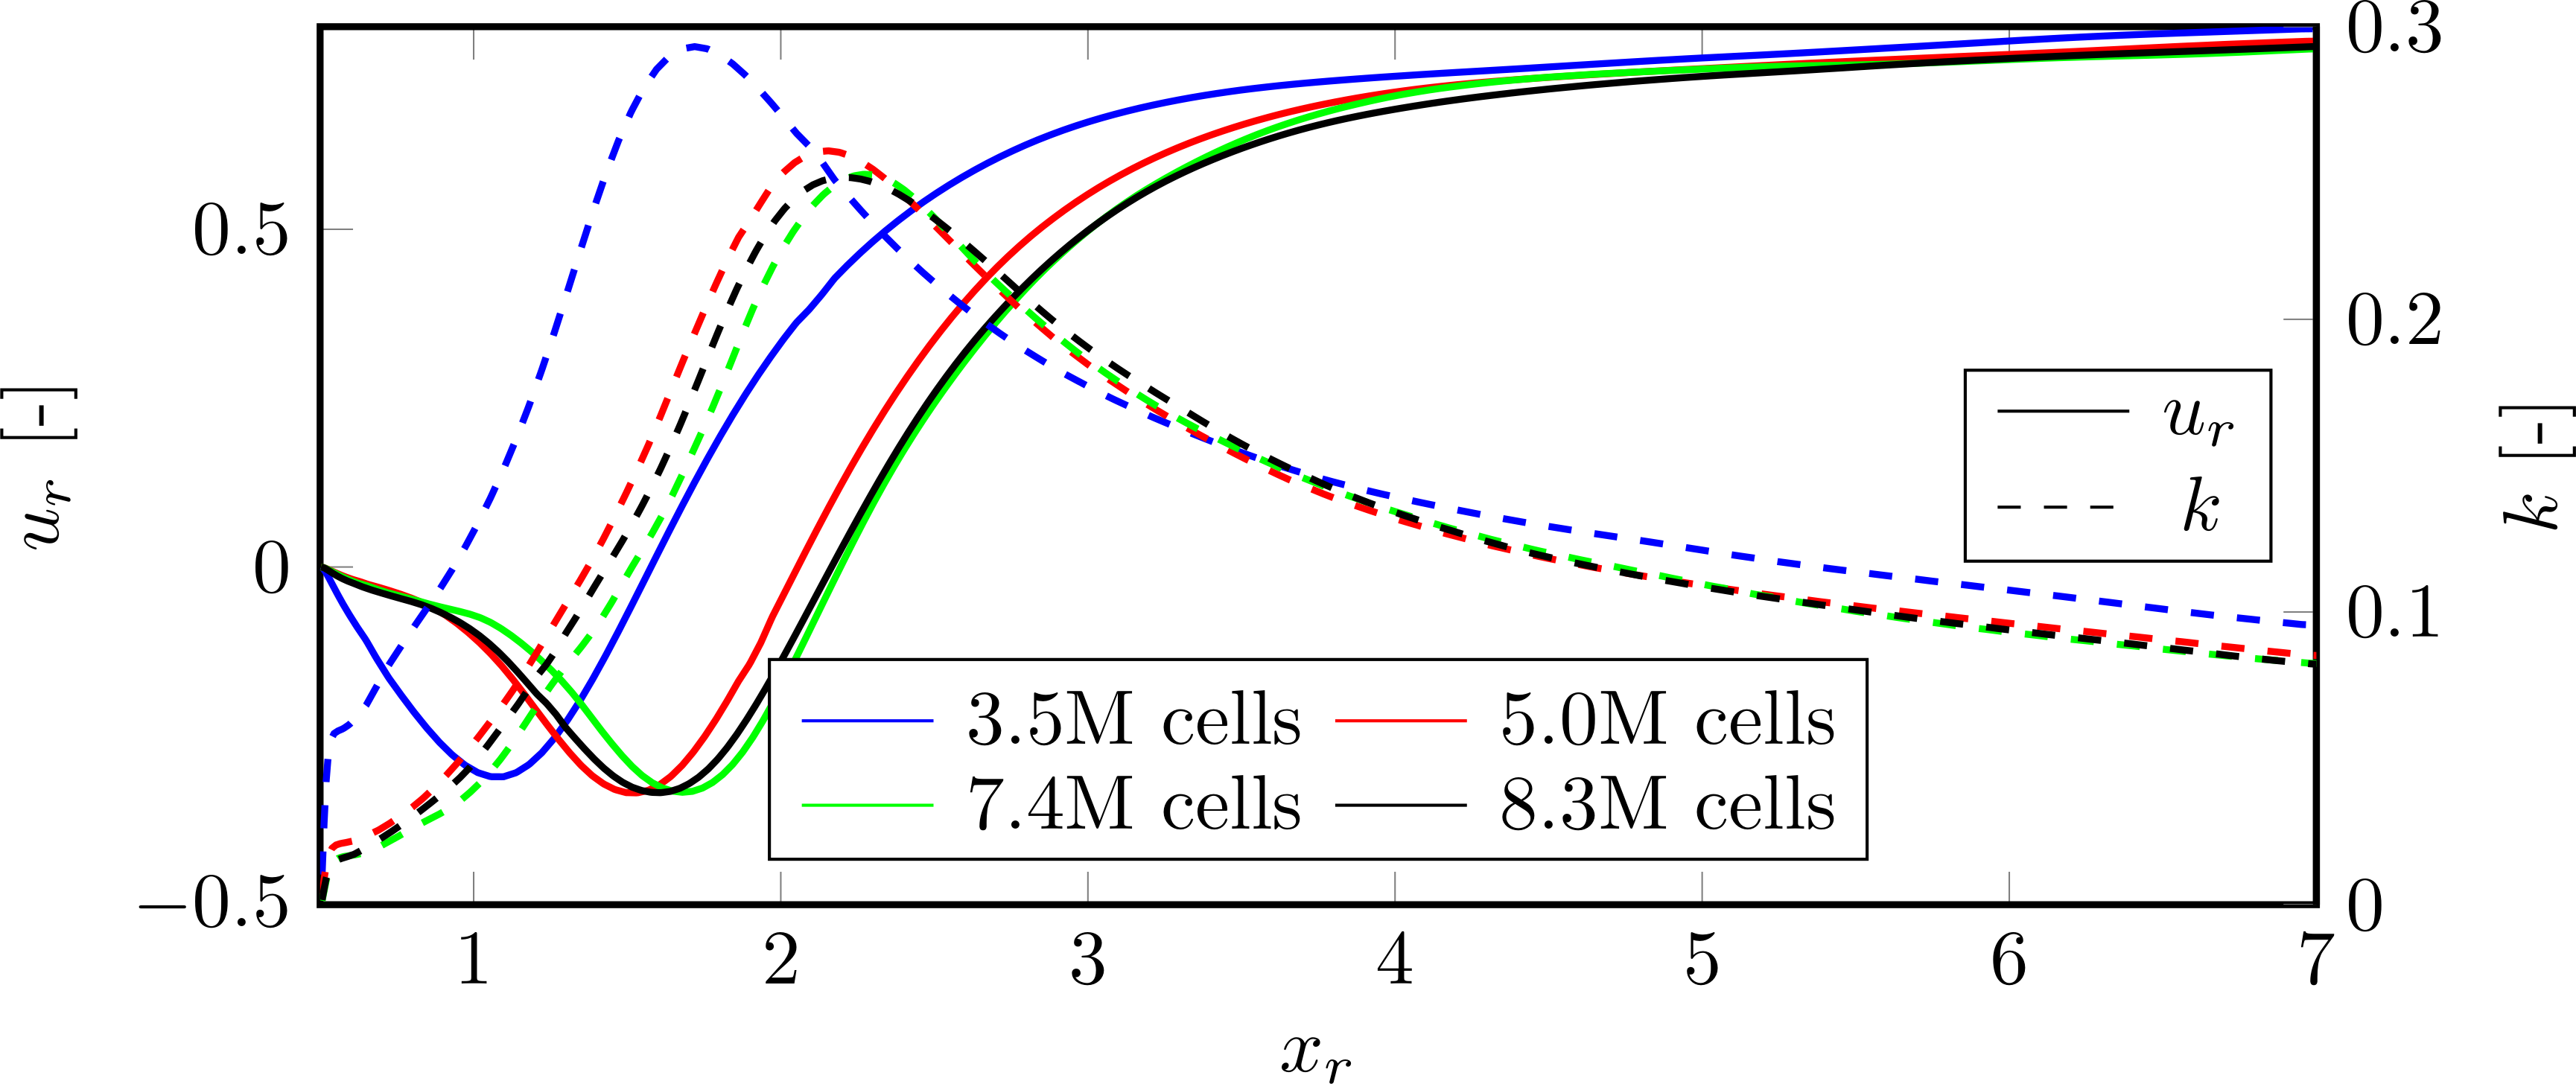
\includegraphics[width=0.98\textwidth]{02_images/00_export/figure3.png}
    \caption{Comparison of the scaled mean flow stream-wise velocity $u_r$ and turbulence kinetic energy $k$ profiles on line $\sigma$ in PoM1 for computational meshes comprising 3.5, 5.0, 7.4 and 8.3 million FV cells.}
    \label{fig:meshIndep}
\end{figure}
In order to obtain mesh resolution independent results, the simulation of flow around a cylinder was repeated four times on four different meshes with varying cell size. In Figure~\ref{fig:meshIndep}, a comparison of the {scaled} mean stream-wise velocity component, $u_r = u/u_{\mathrm{in}}$, and turbulence kinetic energy $k$ profiles on line
\begin{equation}
    {\sigma = \{(x_r,y_r,z_r)\in\mathbb{R}^{3}:x_r\in [0.5,7],\,y_r = 0,z_r=0\}}
\end{equation}
are given for meshes comprising $3.5$, $5.0$, $7.4$ and $8.3$ million{s of} finite volume cells. Increasing number of cells in computational mesh and consequent shrinking of the cell size gradually leads to more similar results. {The mesh with 7.4 million of cells was selected as the one providing a suitable trade-off between the simulation accuracy and overal computational costs. Thus, } all the results presented in \nameref{sec:resultsAndDisc} section are computed on {this mesh}.




